%!TEX root = ../thesis.tex
% Spellcheck ignore
% cSpell:ignore weakfield, intlorgau, gauvslor, atomicmassunit, citep, ifpdf, graphicspath, bigskip, minipage, includegraphics, twolevel, captionof, nano, FWHM, linewidth, electronvolt, Linewidth, nlinewidth, Lorentzian, pagebreak, wrapfigure, photodiode, mathrm, itemsep, extracolsep, toprule, multicolumn, midrule, bottomrule, energylevel, hyperfine, groundstate, nist, groundstates, nonumber, Lorentzians
%*******************************************************************************
%****************************** Second Chapter *********************************
%*******************************************************************************

\ifpdf{}
\graphicspath{{Chapter2/Figs/Raster/}{Chapter2/Figs/PDF/}{Chapter2/Figs/}}
\else
\graphicspath{{Chapter2/Figs/Vector/}{Chapter2/Figs/}}
\fi

\chapter{Absorption of photon by an atom}  %Title of the Second Chapter
The purpose of this section is to outline the basic features observed in saturated absorption
spectroscopy and relate them to simple atomic and laser physics principles.
For this we will follow the guidance of \citep{SAS} and \citep{SAS_appendix}.

A Atomic spectrum is composed of several absorption lines, but usually well 
separated. So if we are close to one line absorption of light by another
line is negligible. In that case the system can be described by a two-level
atom, which we will use in the further sections.


%********************************** % First Section  *************************************
\section{Laser interactions~-~Two-level atom} %Section - 2.1

We begin with the interaction between a laser field and a sample of stationary atoms having
only two possible energy levels. Aspects of thermal motion will be treated subsequently.\\
The difference \(\Delta E = E_1 - E_0\) between the excited state \ket{e} energy \(E_1\) and
ground state \ket{g} energy \(E_0\) is used with Planck's law to determine the photon frequency
\(\nu \) associated with transitions between the two states:
\begin{align}
    \Delta E = h \nu_0
\end{align}
There are three transition processes involving atoms and laser fields:
\bigskip

\begin{minipage}[c][][c]{.35\textwidth}
\begin{itemize}
\item[(1)] absorption
\item[(2)] spontaneous emission
\item[(3)] stimulated emission
\end{itemize}
\end{minipage}
\hfill
\begin{minipage}[c]{.55\textwidth}
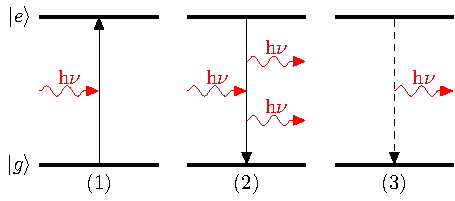
\includegraphics[width=\textwidth]{twolevel}
\captionof{figure}{Two-level atom model}
\end{minipage}
\bigskip

We consider spontaneous emission first~--~a process characterized by a transition rate or probability
per unit time for an atom in the excited state to decay to the ground state. This transition rate will 
be denoted \(\Gamma_\omega \) and is about \(2\pi\cdot \SI{1.3}{\mega\hertz} \) for the rubidium levels
studied here. \\
In the absence of an external field, any initial population of excited state atoms would decay exponentially
to the ground state with a mean life time \(\Delta t = 1/\Gamma_\omega \approx \SI{122}{\nano\second} \).
In the rest frame of the atom, spontaneous photons are emitted in all directions with an energy spectrum
having a mean \(E=h\nu_0 \) and a full width at half maximum (FWHM) \(\Delta E \) given by the
Heisenberg uncertainty principle \(\Delta E \Delta t = \hbar \) or \(\Delta E = \Gamma_\omega\hbar \).
Expressed in frequency units, the FWHM is called the \textit{natural linewidth} and given the symbol
\(\Gamma_\nu \). Thus
\begin{align}\label{eq:gamma_relation}
    \Gamma_\nu = \frac{\Gamma_\omega}{2\pi}
\end{align}
For our rubidium levels, \(\Delta E \approx 5.4\cdot \SI{e-9}{\electronvolt} \) or \(\Gamma_\nu\approx \SI{1.3}{\mega\hertz} \). \\ 
The stimulated emission and absorption processes are also described by a transition rate~--~a single rate
giving the probability per unit time for a ground state atom to absorb a laser photon or for an excited
state atom to emit a laser photon. The stimulated transition rate is proportional to the laser intensity
\textit{I} (SI units of \si{\watt\per\meter\squared}) and is only significantly different from zero when
the laser frequency \(\nu \) is near the resonance frequency \(\nu_0 \). This transition rate will be denoted
\(\alpha I \), where 

\begin{minipage}[c][][c]{.45\textwidth}
\begin{align}
    \alpha = \alpha_0 \mathcal{L}(\nu,\nu_0)
\end{align}
and
\begin{align}
    \mathcal{L}(\nu,\nu_0) &= \frac{1}{ 1+4 {(\nu-\nu_0)}^2 / {\Gamma_\nu}^2 }
\end{align}
\end{minipage}
\hfill
\begin{minipage}[c]{.45\textwidth}
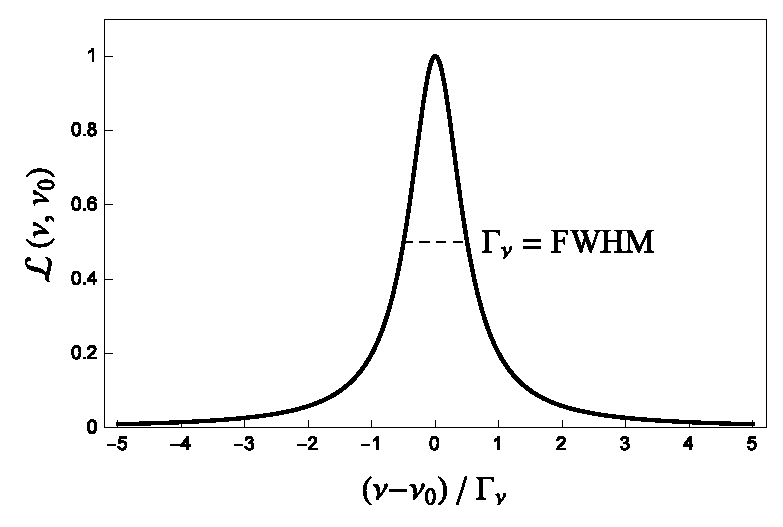
\includegraphics[width=\textwidth]{nLinewidth}
\captionof{figure}{\label{fig:nlinewidth} The Lorentzian line shape profile for resonance absorption}
\end{minipage}
\bigskip

gives the \textit{Lorentzian} frequency dependence as shown in Fig.~\ref{fig:nlinewidth}.
\(\mathcal{L}(\nu,\nu_0) \) also describes the spectrum of radiation from spontaneous emission
and the width \(\Gamma_\nu \) is the same for both cases. The maximum transition rate 
\(\alpha_0 I \) occurs right on resonance (\(\nu~=~\nu_0 \)).\\
The value of \(\Gamma_\omega / \alpha_0 \) defines the saturation intensity \(I_{s} \) of the
atoms. Its significance is that when the laser intensity is equal to the saturation intensity,
excited state atoms are equally likely to decay by stimulated emission or by spontaneous emission.
\pagebreak

%********************************** % Second Section  *************************************
\section{Basic laser absorption spectroscopy}   %Section - 2.2

\begin{wrapfigure}{R}{.5\textwidth}
    \centering
    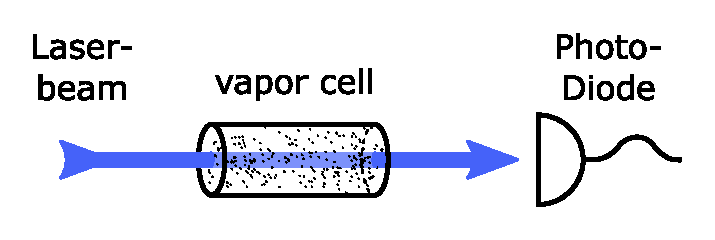
\includegraphics[width=0.45\textwidth]{absorption_spectroscopy_theory}    
    \caption{\label{fig:absorption_spectroscopy} Basic arrangement for ordinary laser absorption spectroscopy.}
\end{wrapfigure}

The basic arrangement for ordinary laser absorption spectroscopy through a gaseous sample is shown in
Fig.~\ref{fig:absorption_spectroscopy}. A laser beam passes through the vapor cell and its intensity is measured
by a photodiode detector as the laser frequency \(\nu \) is scanned through the natural
resonance frequency. \\
When a laser beam propagates through a gaseous sample, the two stimulated transition processes change the intensity
of the laser beam and affect the density of atoms in the ground and excited states. To get a better understanding 
of absorption spectroscopy we begin with the basic equation describing how the laser intensity changes as it 
propagates through the sample and then continue with the effects of Doppler shifts and population changes. 

%********************************** % Third Section  **************************************
\section{Laser absorption} %Section - 2.3

Because of stimulated emission and absorption, the laser intensity \(I(x) \) varies as it propagates from \(x \) to
\(x~+~\mathrm{d}x \) in the medium. The following equation describes this process:
\begin{align} \label{eq:Int}
    I(x+\mathrm{d}x)-I(x) = - I(x) h\nu \alpha n_0  (P_0-P_1) \mathrm{d}x 
\end{align}
where:

\begin{itemize}
    \setlength{\itemsep}{0ex}
    \item[\(n_0\)]\ldots~atom density 
    \item[\(n_0 P_0\)]\ldots~proportion of atoms in \ket{g}
    \item[\(n_0 P_1\)]\ldots~proportion of atoms in \ket{e}
\end{itemize}

Equation~\ref{eq:Int} leads to
\begin{align}
    \frac{ \mathrm{d}I }{ \mathrm{d}x } = -\kappa I
\end{align}
where the \textit{absorption coefficient} (fractional absorption per unit length)
\begin{align}\label{eq:kappa}
    \kappa = h\nu n_0 \alpha (P_0-P_1)
\end{align}

The proportionality to \(P_0-P_1 \) arises from the competition between stimulated emission and absorption
and it is important to appreciate the consequences. If there are equal numbers of atoms in the ground and
excited state (\(P_0-P_1=0\)), laser photons are as likely to be emitted by an atom in the excited state as
they are to be absorbed by an atom in the ground state and there will be no attenuation of the incident beam.
The attenuation maximizes when all atoms are in the ground state (\(P_0-P_1=1\)) because only upward 
transitions would be possible. And the attenuation can even reverse sign (become an amplification as it does
in laser gain media) if there are more atoms in the excited state (\(P_0>P_1\)).

%********************************** % Fourth Section  *************************************
\section{Doppler shifts}  %Section - 2.4

Atoms in a vapor cell move randomly in all directions with each component of velocity having a distribution
of values. Only the component of velocity parallel to the laser beam direction will be important when taking
into account Doppler shifts and it is this component we refer to with the symbol \(v \). The density of atoms
\(\dd n \) in the velocity group between \(v \) and \(v+\dd v \) is given by the Boltzmann velocity
distribution:
\begin{align}
    \dd n = n_0 \sqrt{ \frac{m}{2\pi k_B T} } \exp{ \left( -\frac{mv^2}{2 k_B T} \right ) } \dd v
\end{align}
With a standard deviation given by:
\begin{align}
    \sigma_v = \sqrt{\frac{k_B T}{m}}
\end{align}
This is just a standard Gaussian distribution
\begin{align}
    \dd n = n_0 \frac{1}{\sqrt{2\pi}\sigma_v}  \exp{ \left( -\frac{v^2}{2 {\sigma_v}^2} \right ) } \dd v
\end{align}
with a mean of zero~--~indicating the atoms are equally likely to be going in either direction. It is properly
normalized so that the integral over all velocities (\(-\infty \rightarrow \infty) \) is \(n_0 \), the overall
atom density. \\
Atoms moving with a velocity \(v \) see the laser beam Doppler shifted by the amount \(\nu(v/c) \). We will
take an equivalent, alternate view that atoms moving with a velocity \(v \) have a Doppler shifted resonance
frequency
\begin{align}\label{eq:nu_shift}
    \nu'_0 = \nu_0 \left ( 1 + \frac{v}{c} \right)
\end{align}
in the lab frame. The sign has been chosen to be correct for a laser beam propagating in the positive direction
so that the resonance frequency is blue shifted to higher frequencies if \(v \) is positive and red shifted if
\(v \) is negative.\\
The absorption coefficient \(\dd\kappa \) from a velocity group \(\dd n \) at a laser frequency 
\(\nu \) is then obtained from Eq.~\ref{eq:kappa} by substituting \(\dd n \) for \(n_0 \) and by adjusting
the Lorentzian dependence of \(\alpha \) so that it is centered on the Doppler shifted resonance frequency
\(\nu'_0 \) (Eq.~\ref{eq:nu_shift}).
\begin{align}
    \dd\kappa = h\nu \alpha_0(P_0-P_1) \mathcal{L}(\nu,\nu'_0) \dd n
\end{align}
The absorption coefficient from all atoms is then found by integrating over all velocity groups.

%********************************** % Fifth Section  *************************************
\section{\label{sec:weakfield}Absorption coefficient~-~weak field}   %Section - 2.5

We treat the weak-laser case first where we have a very low intensity compared to \(I_\mathrm{s}\) and
therefore nearly all atoms will be in the ground state, i.e., \(P_0-P_1 = 1 \) so that
\begin{align}
    \mathrm{d}\kappa = h\nu \alpha_0 n_0 \frac{1}{\sqrt{2\pi}\sigma_v} \mathcal{L}(\nu,\nu'_0) \exp{ \left( -\frac{v^2}{2 {\sigma_v}^2} \right ) } \dd v
\end{align}
and
\begin{align}
    \kappa = \underbrace{ h\nu \alpha_0 n_0 \frac{1}{\sqrt{2\pi}\sigma_v} }_{\beta} 
    \int\limits_{-\infty}^{\infty} \frac{1}{ 1+4 {\left [\nu-\nu_0\left ( 1 + \frac{v}{c} \right) \right] }^2 / {\Gamma_\nu}^2 } 
    \exp{ \left (-\frac{v^2}{ 2{\sigma_v}^2 }\right ) } \dd v
\end{align}
After the variable transformation
\begin{align*}
\left |~
    \begin{aligned}
        \nu'_0 =&~\nu_0\left ( 1+ \frac{v}{c} \right) \\
        v =&\left ( \frac{\nu'_0}{\nu_0} - 1 \right) c =\left( \frac{\nu'_0 - \nu_0}{\nu_0} c\right) \\
        \dd v =&~\frac{c}{\nu_0}~\dd \nu'_0
    \end{aligned}
~\right |~ = \beta~\frac{c}{\nu_0} \int\limits_{-\infty}^{\infty} \frac{1}{ 1+4 {(\nu-\nu'_0)}^2 / {\Gamma_\nu}^2 } 
\exp{ \left ( -\frac{{(\nu'_0 - \nu_0)}^2 c^2 }{2 {\nu_0}^2 {\sigma_v}^2 } \right )} \dd \nu'_0
\end{align*} 

and substitution \(\sigma_\nu = \frac{\nu_0}{c} \sigma_v \) we get
\begin{align}
    = \beta~\frac{c}{\nu_0} \int\limits_{-\infty}^{\infty} \frac{1}{ 1+4 {(\nu-\nu'_0)}^2 / {\Gamma_\nu}^2 } 
\exp{ \left ( -\frac{{(\nu'_0 - \nu_0)}^2 }{2 {\sigma_\nu}^2 } \right )} \dd \nu'_0 \label{eq:intlorgau}
\end{align}
Now we compare the width parameters from the Lorentzian (see table~\ref{table:iso_prop}) with the Gaussian function for a temperature of \SI{100}{\degreeCelsius}:

\begin{minipage}[c][][c]{.45\textwidth}
\centering
\begin{align*}
    &\sigma_\nu = \frac{c}{\lambda_\mathrm{D2}} \sqrt{\frac{k_B T}{m_{Rb85} c^2}} \approx \SI{455}{\mega\hertz} \\ \\
    &\Gamma_{\nu,\mathrm{D2}} = \SI{0.282}{\mega\hertz} \\ \\
    &\Rightarrow \Gamma_{\nu,\mathrm{D2}} \ll 2\cdot\sigma_\nu
\end{align*}
\end{minipage}
\hfill
\begin{minipage}[c]{.45\textwidth}
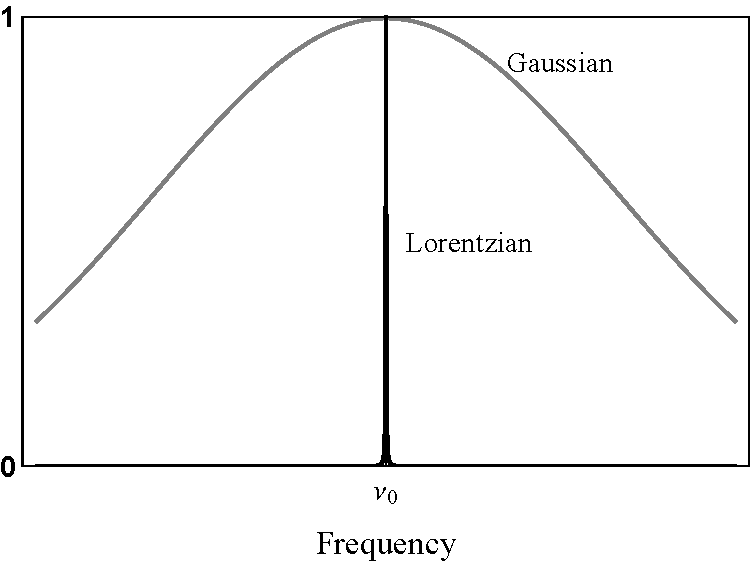
\includegraphics[width=\textwidth]{gauvslor}
\captionof{figure}{\label{fig:gauvslor} The Lorentzian compared to the Gaussian profile}
\end{minipage}
\bigskip

As we can see the Lorentzian function is significantly different from zero only within a very narrow range.
Consequently the Gaussian remains relatively constant over the width of \(\Gamma_{\nu,\mathrm{D2}} \).
Therefore Eq.~(\ref{eq:intlorgau}) can be accurately determined as the integral of the Lorentzian times the 
value of the exponential at \(\nu'_0 = \nu \):
\begin{align}
    = \beta~\frac{c}{\nu_0} \exp{ \left ( -\frac{{(\nu - \nu_0)}^2 }{2 {\sigma_\nu}^2 } \right )} 
    \int\limits_{-\infty}^{\infty} \frac{1}{ 1+4 {(\nu-\nu'_0)}^2 / {\Gamma_\nu}^2 } \dd \nu'_0
\end{align}
and with the solution of the Lorentzian integral
\begin{align}
    \int\limits_{-\infty}^{\infty} \mathcal{L}(\nu,\nu'_0) \dd \nu'_0 = \frac{\pi \Gamma_\nu}{2}
\end{align}
we finally get the absorption coefficient in a weak field
\begin{align}\label{eq:kappa_weakfield}
    \kappa = \kappa_0 \exp{ \left ( -\frac{{(\nu - \nu_0)}^2 }{2 {\sigma_\nu}^2 } \right )} ~~\text{with}~~ \kappa_0 = h\nu \alpha_0 n_0 \frac{1}{\sqrt{2\pi}\sigma_\nu} \frac{\pi \Gamma_\nu}{2}
\end{align}


%********************************** % Sixth Section  *************************************
\section{Population}   %Section - 2.6
Before we can determine the general case of the absorption coefficient we need an expression for \(P_0-P_1 \).
For that we have to take into account the changes to the ground and excited state populations arising
from a laser beam propagating through the cell. The rate equations for the ground and excited state
probabilities or fractions become:
\begin{align}
    \frac{\mathrm{d}P_0}{\mathrm{d}t} &= \Gamma_\omega P_1 - \alpha I (P_0-P_1) \nonumber \\
    \frac{\mathrm{d}P_1}{\mathrm{d}t} &= -\Gamma_\omega P_1 + \alpha I (P_0-P_1)
\end{align} 
where the first term on the right in each equation arises from spontaneous emission and the second term
arises from stimulated absorption and emission.\\
Considering \(P_0+P_1=1 \) and the steady state condition
\begin{align}
    \frac{\mathrm{d}P_0}{\mathrm{d}t} = \frac{\mathrm{d}P_1}{\mathrm{d}t} = 0
\end{align}
we get for the populations
\begin{align}
        P_0 = \frac{\Gamma_\omega + \alpha I}{\Gamma_\omega + 2 \alpha I}~; \qquad
        P_1 = \frac{\alpha I}{\Gamma_\omega + 2 \alpha I}
\end{align}
which leads to
\begin{align}
    (P_0-P_1) = \frac{\Gamma_\omega}{\Gamma_\omega + 2 \alpha I} 
\end{align}
As we can see the population difference is dependent on \(\Gamma_\omega \) (spontaneous decay rate),
which is related to the \textit{Lorentzian width parameter} \(\Gamma_\nu \).
To combine the Lorentzians in \(\alpha \) and \(P_0-P_1 \) we rewrite both expressions with 
Eq.~\ref{eq:gamma_relation} and \(\Delta\nu = 2(\nu-\nu_0) \):
\begin{align}
    \alpha = \alpha_0\frac{1}{ 1+ \Delta\nu^2 / {\Gamma_\nu}^2 } 
                           = \alpha_0\frac{\Gamma_\nu^2}{\Gamma_\nu^2 + \Delta\nu^2}~; \qquad
    (P_0-P_1) = \frac{2\pi\Gamma_\nu}{2\pi\Gamma_\nu + 2 \alpha I}
\end{align}
and get
\begin{align}
    (P_0-P_1)\alpha = \frac{2\pi\Gamma_\nu}{2\pi\Gamma_\nu + 2I \alpha_0\frac{\Gamma_\nu^2}{\Gamma_\nu^2 + \Delta\nu^2}}~ 
    \alpha_0\frac{\Gamma_\nu^2}{\Gamma_\nu^2 + \Delta\nu^2} = \frac{\alpha_0\pi\Gamma_\nu^2}{\pi(\Gamma_\nu^2 + \Delta\nu^2)+I\alpha_0\Gamma_\nu}
\end{align}
dividing with \(\pi\Gamma_\nu \) and substitute in the denominator \(\alpha_0 \) with the definition of \( I_s = 2\pi\Gamma_\nu / \alpha_0 \) leads to
\begin{align}
    \alpha_0 \frac{1}{1 + \frac{\Delta\nu^2}{\Gamma_\nu} + \frac{2I}{I_s} } = \frac{\alpha_0}{(1 + \frac{2I}{I_s})}~\frac{1}{1+ \frac{\Delta\nu^2}{\Gamma_\nu^2(1 + \frac{2I}{I_s})}}
\end{align}
with the definition of the power-broadened \textit{width parameter}
\begin{align}
    \Gamma'_\nu = \Gamma_\nu \sqrt{1 + 2I/I_s}
\end{align}
we obtain
\begin{align}
    (P_0-P_1)\alpha = \frac{\alpha_0}{(1 + \frac{2I}{I_s})}~\mathcal{L}'(\nu,\nu_0)~~\text{and}~~\mathcal{L}'(\nu,\nu_0)= \frac{1}{1+ \frac{{4(\nu-\nu_0)}^2}{{\Gamma'_\nu}^2}}
\end{align}
\pagebreak
%********************************** % Seventh Section  *************************************
\section{Absorption coefficient~-~general case}  %Section - 2.7
For the general case we take now into account the velocity groups and their corresponding Doppler 
shifts for the case \(P_0-P_1 \neq 1 \) and therefore 
\begin{align}
    \mathrm{d}\kappa = h\nu n_0 \frac{\alpha_0}{(1 + \frac{2I}{I_s})} \frac{1}{\sqrt{2\pi}\sigma_v} \mathcal{L}'(\nu,\nu'_0) \exp{ \left( -\frac{v^2}{2 {\sigma_v}^2} \right ) } \dd v
\end{align}
and
\begin{align}
    \kappa = h\nu n_0 \frac{\alpha_0}{(1 + \frac{2I}{I_s})} \frac{1}{\sqrt{2\pi}\sigma_v} 
    \int\limits_{-\infty}^{\infty} \frac{1}{ 1+4 {\left [\nu-\nu_0\left ( 1 + \frac{v}{c} \right) \right] }^2 / {\Gamma'_\nu}^2 } 
    \exp{ \left (-\frac{v^2}{ 2{\sigma_v}^2 }\right ) } \dd v
\end{align}
The calculation can be performed as in Section~\ref{sec:weakfield} with the only addition of the
the power-broadened \textit{width parameter} \(\Gamma'_\nu \). This leads to
\begin{align}
    \kappa'_0 &= h\nu n_0 \frac{\alpha_0}{(1 + \frac{2I}{I_s})} \frac{1}{\sqrt{2\pi}\sigma_\nu} \frac{\pi \Gamma'_\nu}{2}
    = h\nu n_0 \frac{\alpha_0}{(1 + \frac{2I}{I_s})} \frac{1}{\sqrt{2\pi}\sigma_\nu} \frac{\pi \Gamma_\nu}{2} \sqrt{1+ \frac{2I}{I_s}} \nonumber \\
    &= h\nu n_0 \frac{\alpha_0}{\sqrt{1 + \frac{2I}{I_s}}} \frac{1}{\sqrt{2\pi}\sigma_\nu} \frac{\pi \Gamma_\nu}{2}
    = \frac{\kappa_0}{\sqrt{1 + \frac{2I}{I_s}}}
\end{align}
and subsequently
\begin{align}
    \kappa = \kappa'_0 \exp{ \left ( -\frac{{(\nu - \nu_0)}^2 }{2 {\sigma_\nu}^2 } \right )} \label{eq:kappa_general}
\end{align}

\pagebreak
%********************************** % Seventh Section  *************************************
\section{Non-linear differential equation}  %Section - 1.7

\pagebreak

\section{Data table}

\begin{table}[h]
\centering
\begin{tabular*}{0.9\textwidth}{@{\extracolsep{\fill} }l l c c}
\toprule
& & \multicolumn{2}{c}{Rubidium} \\
\midrule
Isotope & [1] & 85 & 87 \\
Atomic mass & [\si{\atomicmassunit}] & 84.911794 & 86.909187 \\
\num{e-25} & [\si{\kilogram}] & 1.40999 & 1.44316 \\
Abundance & [\si{\percent}] & 72.17 & 27.83 \\
Spin I & [1] & \(\sfrac{5}{2}\) & \(\sfrac{3}{2}\) \\
Lifetime \(6^{2}P_{3/2}\) & \([ \si{\nano\second} ]\) & & \num{112} \\
Lifetime \(6^{2}P_{1/2}\) & \([ \si{\nano\second} ]\) & & \num{125} \\
Wavelength D1-Line (\(6^{2}P_{1/2} \rightarrow 5^{2}S_{1/2}\)) & [\si{\nano\meter}] & 421.5524 & \\
Wavelength D2-Line (\(6^{2}P_{3/2} \rightarrow 5^{2}S_{1/2}\)) & [\si{\nano\meter}] & 420.1792 & \\
A\(_{\mathrm{ki,D1}},~\Gamma_{\omega,\mathrm{D1}}\) & \([ \si{\per\second} ] \) & \num{1.50e6} & \\
A\(_{\mathrm{ki,D2}},~\Gamma_{\omega,\mathrm{D2}}\) & \([ \si{\per\second} ] \) & \num{1.77e6} & \\
Natural linewidth \(\Gamma_{\nu,\mathrm{D1}}\) & \([ \si{\mega\hertz} ]\) & \num{0.239} & \\
Natural linewidth \(\Gamma_{\nu,\mathrm{D2}}\) & \([ \si{\mega\hertz} ]\) & \num{0.282} & \\
\bottomrule
\end{tabular*}
\caption{\label{table:iso_prop}Properties of rubidium isotopes}
\end{table}
\pagebreak

%********************************** % Eighth Section  *************************************

\section{D2 line} %Section - 1.2 

\begin{figure}[h]
\centering
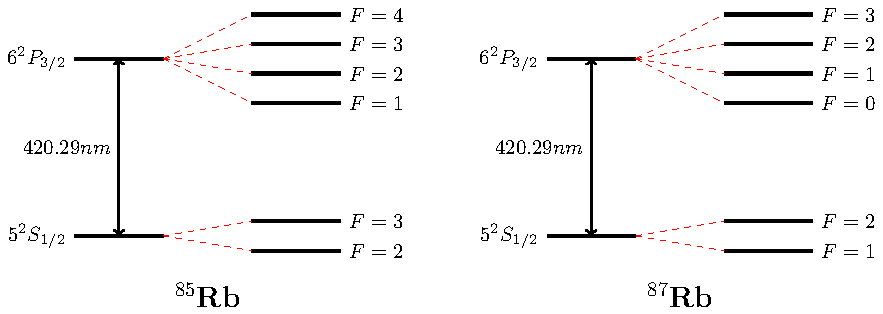
\includegraphics[width=0.9\textwidth]{energylevel}
\caption{\(5^{2}S_{1/2} \rightarrow 6^{2}P_{3/2}\) transition of \(^{85}\)Rb and \(^{87}\)Rb with corresponding hyperfine structure}    
\end{figure}

\vspace{\fill}

The transition of interest is, as we have discussed before, the \(5^{2}S_{1/2} \rightarrow 6^{2}P_{3/2}\) of rubidium. As known rubidium
occurs in two isotopes, \(^{85}\)Rb and \(^{87}\)Rb.
As we can see both isotopes have the same transition energy, but due to the different spin I (see table:~\ref{table:iso_prop}) we get
different energy levels for the groundstate \citep{nist_asd}. This is the reason why we witness four Doppler peaks in our spectrum.
\bigskip

\textbf{Caution:} Both figures below show the correct correlation between energy and isotopes. The reason for this is that the spectrum
shows transition energy and the other one the specific energy levels.

\vspace{\fill}

\begin{figure}[h]
\centering
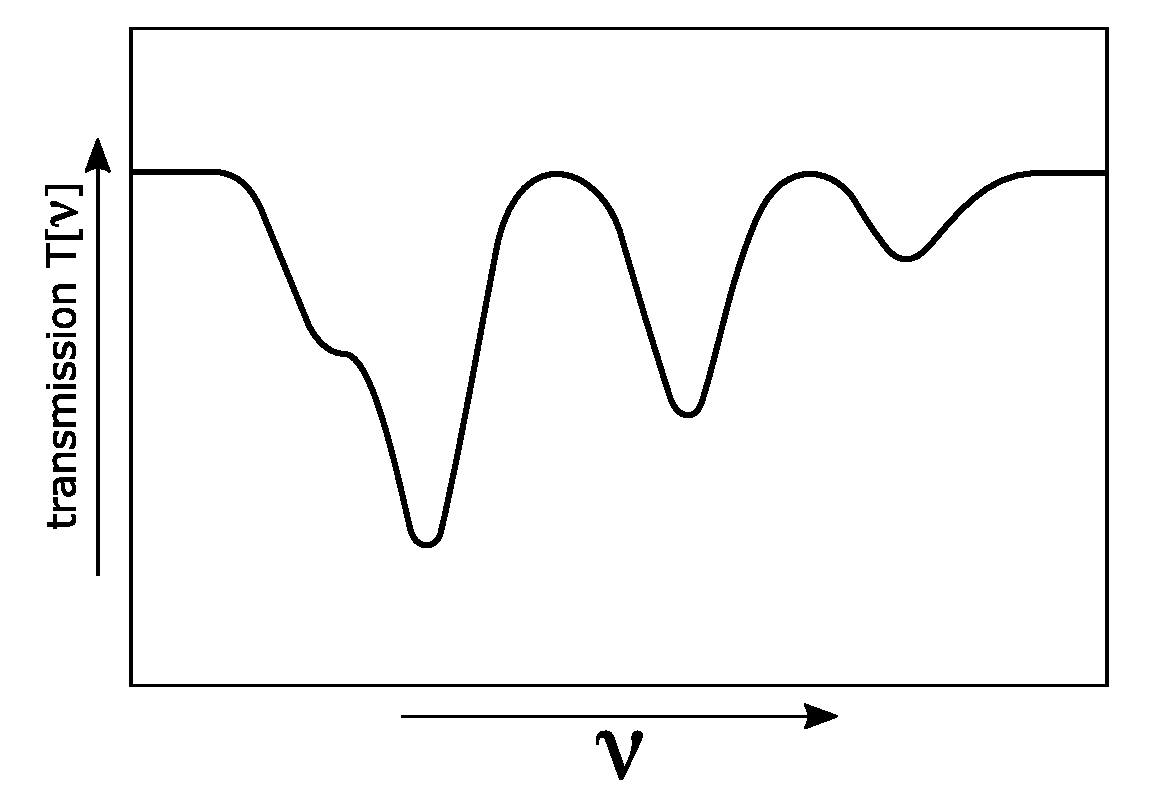
\includegraphics[width=0.6\textwidth]{spectrum_doppler}
\caption{\label{fig:doppler}Doppler spectrum of D2 line} 
\end{figure}

\vspace{\fill}

\begin{figure}[ht]
\centering
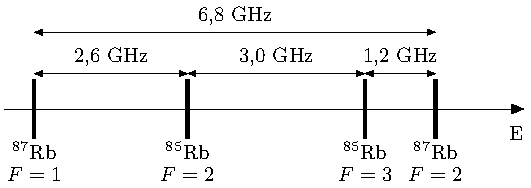
\includegraphics[width=0.6\textwidth]{groundstate}
\caption{\label{fig:gap}Relative energy gaps of the groundstates between both isotopes} 
\end{figure}